\DiaryEntry{Upcoming Ideas...}{}{}

\subsection{Making a denominator square-root free.}

\bee
\frac{1}{1 + \sqrt{2}} = \frac{1 - \sqrt{2}}{(1 + \sqrt{2})(1 - \sqrt{2})} = \frac{1 - \sqrt{2}}{1 - 2} = \sqrt{2} - 1
\eee

Based on $(a-1)(a+1) = a^2 - 1$.

A similar idea is to make the denominator real,

\bee
\frac{1}{1-j} = \frac{1+j}{(1-j)(1+j)} = \frac{1+j}{(1-j)(1+j)} = \frac{1+j}{2}
\eee


\subsection{Graph / Tree traversal}

Actually, two things. Numerb one: The DFS algorithm \ref{2020-02-27:entry} is recursive. There is, however, also an iterative version available which uses a stack. Implement this algorithm.

Number two: Both BFS and DFS simplify in case of a tree as it is a graph without cycles. Show how the algs simplify in this case.


\subsection{Inequalities and Squareroots}

Prove that $0 < 11 - 6 \sqrt{3} < 1$. We have the following reasoning:

\begin{align*}
  &121 > 108 > 100 \\
  &\sqrt{121} > \sqrt{108} > \sqrt{100} \\
  &11 > 6 \sqrt{3} > 10 \\
  &-11 < -6 \sqrt{3}  < -10
\end{align*}

The square root is a convex function, therefore from $A > B$ follows $\sqrt{A} > \sqrt{B}$ which explains the step from the first to second line.

Adding $11$ to the last line yields

\bee
0 < 11 - 6 \sqrt{3} < 1 \qed
\eee

Also interesting is to bound a square root between integers which differ by one; e.g. $A < \sqrt{37} < B$. We can bound this as follows

\begin{align*}
  &\sqrt{36} < \sqrt{37} < \sqrt{49} \\
  & 6 < \sqrt{37} < 7
\end{align*}

For the lower / upper bound we use the ``closest'' square number. The root then gives integers and the bounds differ by $1$ as requested. This holds for all numbers in between; i.e. we have

\bee
6 < \sqrt{37} \cdots \sqrt{48} < 7
\eee


\subsection{Distance Point - Random Point}

Here we have one fixed point $P(x_P,0)$ and ask for the distance $d$ to another point $Q$ located randomly inside the unit circle / box. The distance $d$ is random and given by

\bee
d = \sqrt{(x_p - x)^2 + y^2}
\eee

where $(x,y)$ are the coordinates of $Q$. In case of a unit box, they are distributed according to

\bee
x,y \sim \Uc(-1,1)
\eee

in case of a unit circle, they are constrained by $x^2 + y^2 \leq 1$. According to \href{https://stats.stackexchange.com/questions/481543/generating-random-points-uniformly-on-a-disk}{this} Stackoverflow answer, the distributions of $x$ and $y$ are a bit more tricky...

The expected distance $E(d)$ is then given by

\bee
E(d) = \int_{x,y} d f_x(x) f_y(y) dx dy
\eee

where $f_x(x), f_y(y)$ are the distributions of $x$ and $y$, respectively. The integrals seem to be rather tricky; even in case of the unit box (where the distribution is simple), I'm not sure if there is a closed-form solution for the double-integral. In case of the unit disc, already the distributions are complex (polar coordinates may help as $\phi$ is uniform in $[0, 2\pi]$ and $r$ is $\sim  r$ in $[0,1]$.

\subsection{Predator-Prey}

See entry \ref{2018-07-30:entry} and extend it to general coefficients,

\begin{align}\label{2018-07-30-eq1}
R' = \frac{dR}{dt} &= \alpha R - \beta RF \nonumber \\
F' = \frac{dF}{dt} &= -\gamma F + \delta RF
\end{align}

We can rewrite the first equation as $R(\alpha - \beta F) = 0$ and obtain two fixed points from it: (i) $R = $, (ii) $F = \alpha/\beta$. We can use the second equation similarly, $F(- \gamma+  \delta R)$ and obtain (i) $F = 0$, (ii) $R = \gamma/\delta$. Therefore, we have two fixed points,

\begin{align}
  &R = F = 0\\
  &R = \gamma / \delta, F = \alpha / \beta
\end{align}

To assess the stability of the fixed points, we calculate the Jacobian $\Jbf$ of the differential equation system \todo{Check!!!},

\bee
\Jbf = \begin{pmatrix} \frac{dR'}{dR} & \frac{dR'}{dF} \\ \frac{dF'}{dR} & \frac{dF'}{dF} \end{pmatrix} = \begin{pmatrix} \alpha - \beta F & - \beta R \\ \delta F & \delta R - \gamma \end{pmatrix}
\eee

Let's consider the fixed point $R = F = 0$ first. For these values, the Jacobian becomes

\bee
\Jbf_1 = \begin{pmatrix} \alpha & 0 \\ 0 & - \gamma \end{pmatrix}
\eee

The eigenvalues are the solution to $|\Jbf_1 - \lambda \Ibf | = 0$. We have

\bee
\begin{vmatrix} \alpha - \lambda & 0 \\ 0 & - \gamma - \lambda \end{vmatrix} = (\alpha - \lambda)(- \gamma - \lambda) = 0
\eee

and therefore the two eigenvalues become $\lambda_1 = \alpha, \lambda_2 = - \gamma$. In our model, the parameters $\alpha$ and $\gamma$ are always greater than zero, and therefore such the sign of the eigenvalues will be different. Hence the fixed point at the origin is a saddle point which is an instable fixed point \todo{is a saddle point always instable?}.

For the other fixed point ($R = \gamma / \delta, F = \alpha / \beta$), the Jacobian becomes

\bee
\Jbf_2 = \begin{pmatrix} \alpha - \beta \alpha / \beta & - \beta \gamma / \delta \\ \delta \alpha / \beta & \delta \gamma / \delta - \gamma \end{pmatrix} = \begin{pmatrix} 0 & - \beta \gamma / \delta \\ \delta \alpha / \beta & 0 \end{pmatrix}
\eee

The eigenvalues of this matrix are given by

\bee
\begin{vmatrix} -\lambda & - \beta \gamma / \delta \\ \delta \alpha / \beta & - \lambda \end{vmatrix} = \lambda^2 - (- \beta \gamma / \delta)(\delta \alpha / \beta) = 0
\eee

From this follows

\bee
\lambda^2 + \alpha \gamma = 0 \rightarrow \lambda_{1,2} = \pm j \sqrt{\alpha \gamma}
\eee

As the eigenvalues are both purely imaginary and conjugate to each other, this fixed point must either be a center for closed orbits in the local vicinity or an attractive or repulsive spiral. In conservative systems, there must be closed orbits in the local vicinity of fixed points that exist at the minima and maxima of the conserved quantity. \todo{Copied from Wikipedia - do not understand completely!}

\begin{figure}[H]
    \centering
    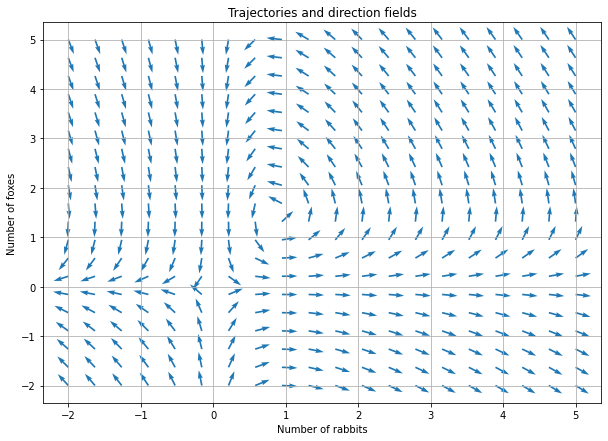
\includegraphics[scale=0.6]{images/predator_prey.png}
\end{figure}


\subsection{Walli's Integral}

Defined as (Nahin, Inside Interesting Integrals, p. 122),

\bee
I(k) = \int_0^1 (x-x^2)^k dx = \int_0^1 x^k (1-x)^k dx = B(k+1, k+1) = \frac{\Gamma(k+1) \Gamma(k+1)}{\Gamma(2k+2)}
\eee

which becomes (for integer-valued $k$)

\bee
I(k) = \int_0^1 (x-x^2)^k dx = \frac{(k!)^2}{(2k+1)!}
\eee

Especially interesting is $k =1/2$. TODO


\subsection{Integral $\log(x)/x^k$}

Start with $k = 2$ and consider the following integral

\bee
I = \int_1^\infty \frac{\log(x)}{x^2}dx
\eee

which we can solve via partial integration: We chose $u=\log(x), v'=1/x^2$ and obtain $u' = 1/x, v = -1/x$ and therefore the integral becomes

\bee
I = - \left. \frac{\log(x)}{x} \right|_1^\infty + \int_1^\infty \frac{1}{x^2} dx = 0 + \left.\left( - \frac{1}{x} \right)\right|_1^\infty = 1
\eee

Interestingly, this can be extended to

\bee
I = \int_1^\infty \frac{\log(x)}{x^k}dx
\eee

Same procedure, $u=\log(x), v'=1/x^k$ and obtain $u' = 1/x, v = \frac{x^{-k+1}}{-k+1}$ and therefore we have

\bee
I = - \left. \frac{x^{-k+1} \log(x)}{-k+1} \right|_1^\infty - \int_1^\infty x^{-1} \frac{x^{-k+1}}{-k+1} dx = 0 - \frac{1}{1-k} \int_1^\infty x^{-k} dx = \frac{1}{(k-1)^2}
\eee

\subsection{Where should I open my restaurant?}

Based on \cite{Kaplan2017}.

A walk on the $\Zc^2$ lattice using only the steps $(0, 1)$, which we call ``North'', and $(1, 0)$, which we call ``East'' is a lattice path.

Question 1: How many lattice paths begin at $(0, 0)$ and end at $(m, n)$?

The path consists of $m$ steps East and $n$ steps North. In total we need to make $m+n$ steps to reach the destination and it does not matter when we go North and East. We therefore have

\bee
{m+n \choose m}
\eee

different lattice paths. A classical application of the binomial.

Question 2: How many of these paths pass through the point $(a, b)$?

We can split the path into two parts: One from $(0,0)$ to $(a,b)$ and one from $(a,b)$ to $(m,n)$. We can apply the same argument from before to each of the two paths and note that we can chose them independently; i.e. we multiply their numbers.

For the first part we have ${a+b \choose a}$ possibilities, for the second one (with $m-a$ steps East and $n-b$ steps North) we have ${m-a+n-b \choose m-a}$ possibilities. Therefore, there are

\bee
{a+b \choose a} {m-a+n-b \choose m-a}
\eee

different lattice paths.

\subsection{TIKZ}

Some text...

\begin{figure}[H]
\centering
\begin{tikzpicture}[transform shape]
  \graph [nodes={circle,draw}] {
    %A -> ["1"] B -> ["2"] C;
    %D -> ["4"] C;
    A -> ["1"] B -> ["2"] C;
    D -> ["4"] C;
    A ->["3", bend left] C;
  };
\end{tikzpicture}
\caption{Example Graph, I.}
\end{figure}


\subsection{Cycle Index - Generating Function}

Based on \cite{Stanley2012}. On p. 24, they define the cycle index as

\bee
Z_n(p_1, \ldots, p_n) = \frac{1}{n!} \sum_p \prod_i t_i^{p_i}
\eee

and provide a generating function for $Z_n$ as

\bee
\sum_n Z_n x^n = \exp \left( t_1 x + t_2 \frac{x^2}{2} + t_3 \frac{x^3}{3} + \cdots \right)
\eee

We need to be a bit careful with the number of terms we want to include in the series expansion; permutations of $N$ elements will have $N$-cycles at most, so we need to go up to $t_N$. As example, for $N=3$ we have

\begin{verbatim}
(%i8)	f1:exp(t1*x + t2*x^2/2 + t3*x^3/3);
(%o8)	%e^((t3*x^3)/3+(t2*x^2)/2+t1*x)
(%i11)	taylor(f1, x, 0, 3);
(%o11)	1+t1*x+((t1^2+t2)*x^2)/2+((t1^3+3*t2*t1+2*t3)*x^3)/6+...
\end{verbatim}

and we can read off the cycle index $Z_3$ as $\frac{1}{6}(t_1^3+3t_1*t_2+2t_3)$. For $N=4$ we need to include another term and we have

\begin{verbatim}
(%i12)	f1:exp(t1*x + t2*x^2/2 + t3*x^3/3 + t4*x^4/4);
(%o12)	%e^((t4*x^4)/4+(t3*x^3)/3+(t2*x^2)/2+t1*x)
(%i14)	taylor(f1, x, 0, 4);
(%o14)	1+t1*x+((t1^2+t2)*x^2)/2+((t1^3+3*t2*t1+2*t3)*x^3)/6+((t1^4+6*t2*t1^2+8*t3*t1+3*t2^2+6*t4)*x^4)/24+...
\end{verbatim}

Therefore the cycle index $Z_4$ is given by $\frac{1}{24}( t_1^4+6t_2 t_1^2+ 8 t_3 t_1+ 3 t_2^2+6 t_4  )$.

With this closed-form expression, we can get some nice results: Let $E_k(n)$ denotes the expected number of $k$-cycles of an $n$-permutation,

\bee
E_k(n) = \frac{1}{n!} \sum_{w \in S_n} c_k(w)
\eee

where $c_k(w)$ denotes the number of $k$-cycles in the permutation $w$. We can write for the expectation

\bee
E_k(n) = \left. \frac{\partial}{\partial t_k} Z_n(t_1, t_2, \ldots, t_n) \right|_{t_i=1}
\eee

Now let's insert our closed form expression for $Z_k$ and we have

\begin{align*}
  \sum_{n \geq 0} E_k(n) x^n &= \frac{\partial}{\partial t_k} \exp\left(  t_1 x + t_2 \frac{x^2}{2} + t_3 \frac{x^3}{3} + \cdots \right) \\
                             &= \frac{x^k}{k} \exp\left(  x + \frac{x^2}{2} + \frac{x^3}{3} + \cdots \right) \\
                             &= \frac{x^k}{k} \exp \log \frac{1}{1-x} \\
                             &= \frac{x^k}{k} \sum_{n \geq 0} x^n
\end{align*}

\todo{not all steps are super clear}. From this we read off

\bee
E_k(n) = \frac{1}{k}
\eee


\subsection{Coin Change and Generating Functions}

Assume we have a coin system with values $a_1, a_2, \ldots, a_n$ and we ask for the number of possibilities $P_V$ we can represent a certain value $V$. This is answered by the generating function,

\bee
\sum_{k \geq 0} P_k x^k = \frac{1}{\prod_i (1-x^{a_i})}
\eee

For example, consider the case with three coins having values $a_1=1, a_2=2, a_3=5$. The generating function becomes

\bee
\sum_{k \geq 0} P_k x^k = \frac{1}{(1-x^1)(1-x^2)(1-x^5)}
\eee

A series expansion (using Maxima) yields

\begin{verbatim}
(%i4)	f:1/((1-x)*(1-x^2)*(1-x^5));
(%o4)	1/((1-x)*(1-x^2)*(1-x^5))
(%i5)	taylor(f, x, 0, 10);
(%o5)	1+x+2*x^2+2*x^3+3*x^4+4*x^5+5*x^6+6*x^7+7*x^8+8*x^9+10*x^10+...
\end{verbatim}

and from this we read off that we can express the value $V=5$ in $P_5=4$ different ways. These are

\bee
1+1+1+1+1, 1+1+1+2, 1+2+2, 5
\eee

Since we have a coin with value $1$, every number is expressible; without such a coin, this is not necessarily possible. This would be seen that the series expansion has ``gaps''. E.g., consider the above example without the one-coin having generating function

\bee
\sum_{k \geq 0} P_k x^k = \frac{1}{(1-x^2)(1-x^5)}
\eee

which can be expanded into 

\begin{verbatim}
(%i6)	f:1/((1-x^2)*(1-x^5));
(%o6)	1/((1-x^2)*(1-x^5))
(%i7)	taylor(f, x, 0, 10);
(%o7)	1+x^2+x^4+x^5+x^6+x^7+x^8+x^9+2*x^10+...
\end{verbatim}

and from this we see that e.g. $V=3$ cannot be expressed.

\paragraph{Interesting Questions.}

\begin{itemize}
  \item Knowing the coin values, can we say whether all numbers can be expressed? In the second example, $V=3$ was not expresible - are there any larger numbers which are not expressible?
  \item With certain coin values, there are larger gaps. Can we say something about the length and density of the gaps? Do they stop for large enough values; i.e. is there a certain value $V^\star$ above which all values are representable? 
\end{itemize}

\begin{verbatim}
(%i21) f:1/(1-x^3)/(1-x^6);
                                       1
(%o21)                         -----------------
                                     3        6
                               (1 - x ) (1 - x )
(%i22) c:taylor(f,x,0,100);
               3      6      9      12      15      18      21      24      27
(%o22)/T/ 1 + x  + 2 x  + 2 x  + 3 x   + 3 x   + 4 x   + 4 x   + 5 x   + 5 x
      30      33      36      39      42      45      48      51       54
 + 6 x   + 6 x   + 7 x   + 7 x   + 8 x   + 8 x   + 9 x   + 9 x   + 10 x
       57       60       63       66       69       72       75       78
 + 10 x   + 11 x   + 11 x   + 12 x   + 12 x   + 13 x   + 13 x   + 14 x
       81       84       87       90       93       96       99
 + 14 x   + 15 x   + 15 x   + 16 x   + 16 x   + 17 x   + 17 x   + . . .
(%i23) makelist(coeff(c,x,n),n,0,100);
(%o23) [1, 0, 0, 1, 0, 0, 2, 0, 0, 2, 0, 0, 3, 0, 0, 3, 0, 0, 4, 0, 0, 4, 
0, 0, 5, 0, 0, 5, 0, 0, 6, 0, 0, 6, 0, 0, 7, 0, 0, 7, 0, 0, 8, 0, 0, 8, 0, 0, 
9, 0, 0, 9, 0, 0, 10, 0, 0, 10, 0, 0, 11, 0, 0, 11, 0, 0, 12, 0, 0, 12, 0, 0, 
13, 0, 0, 13, 0, 0, 14, 0, 0, 14, 0, 0, 15, 0, 0, 15, 0, 0, 16, 0, 0, 16, 0, 
0, 17, 0, 0, 17, 0]
\end{verbatim}

\paragraph{Extensions.} We want to find the number of integer solutions of the equation

\bee
x_1 + x_2 + x_3 =10
\eee

with the constraints $0 \leq x_1 \leq 4$, $0 \leq x_2 \leq 8$, and $4 \leq x_3 \leq 10$. The corresponding generating function is

\bee
F(x) = (1+x^1+x^2+x^3+x^4)(1+x^1+\cdots + x^8)(x^4 + \cdots + x^{10}) = x^4 + \cdots + 25x^{10} + \cdots x^{22}
\eee

and therefore there are $25$ solutions to the equation. If we allow all positive values for $x_1$ (i.e. $0 \leq x_1$, then we have

\bee
F(x) = (1+x^1+x^2+\cdots)(1+x^1+\cdots + x^8)(x^4 + \cdots + x^{10}) = \frac{1}{1-x}(1+x^1+\cdots + x^8)(x^4 + \cdots + x^{10})
\eee

and we can obtain an infinite series expansion according to

\bee
F(x) = x^4 + \cdots + 28 x^{10} + \cdots + 63x^{22} + 63 x^{23} + \cdots
\eee

The first few terms are the same (the removed upper limit of $x_1$ is not relevant), but there are more solutions for the equation and also solutions for values larger then $22$.

Also fun is to include summands which are allowed to be even; this corresponds to a factor of $(1+x^2+x^4 + \cdots)$ in the generating function.


\subsection{Bounding $\pi$}

We consider the following integral,

\bee
\int_0^1 \frac{x^4(1-x)^4}{1+x^2} dx
\eee

We can solve this integral by performing a partial fraction expansion and obtain

\bee
\int_0^1 \frac{x^4(1-x)^4}{1+x^2} dx = \int_0^1 \frac{-4}{1+x^2} + x^6 - 4x^5 + 5x^4-4x^2+4 dx
\eee

The first term yields $-4 \arctan(x)$, the other are trivial polynom integrals. Evaluating the integral at $0$ and $1$, we obtain

\bee
\int_0^1 \frac{x^4(1-x)^4}{1+x^2} dx = \frac{22}{7} - \pi
\eee

Looking at the integrand, we see that it is positive for all $x$ (in particular for $x \in [0,1]$, and integrating a positive function yields a positive value. So we have

\bee
\int_0^1 \frac{x^4(1-x)^4}{1+x^2} dx = \frac{22}{7} - \pi > 0 \rightarrow \pi < \frac{22}{7}
\eee

We can use this result to get a bound for $\pi$ as follows. First we have

\bee
\int_0^1 x^4(1-x)^4 dx = \frac{1}{630}
\eee

and we have the following bounds,

\bee
\int_0^1 \frac{x^4(1-x)^4}{2} dx < \int_0^1 \frac{x^4(1-x)^4}{1+x^2} dx < \int_0^1 x^4(1-x)^4 dx
\eee

The first inequality comes from the fact that $A/2 < A/(1+x^2)$ in the interval $[0,1]$, the second from the fact that $A/(1+x^2) < A$ in the interval $[0,1]$ (with $A = x^4(1-x)^4$.

Solving the integrals yields

\bee
\frac{1}{2 \cdot 630} <  \frac{22}{7} - \pi < \frac{1}{630}
\eee

and we can simplify this to

\bee
\frac{1979}{630} < \pi < \frac{3959}{1260}
\eee

The bound is quite tight; a slightly looser (but nicer) one is

\bee
3 \frac{10}{71} < \pi < 3 \frac{10}{70}
\eee

\subsection{Joining (overlapping) Intervals}

We are given $N$ intervals $[a_1; b_1] \ldots [a_N; b_N]$ of which some are overlapping. We want to determine the smallest set of intervals covering the same ranges as the original intervals.

The algorithm of joining the intervals is as follws:

\begin{itemize}
  \item Order the intervals by $a_k$.
  \item If the first and second interval overlap (that is $[a_1; b_1] \cap [a_2; b_2] \neq 0$), then join them into a new interval $[a;b]$ with $a = \min a_1, a_2$ and $b = \max b_1, b_2$.
  \item If the next interval does not overlap with $[a;b]$, emit $[a;b]$ as part of the solution. Otherwise join $[a;b]$ with the next interval.
  \item Continue until all intervals have been processed.
\end{itemize}


\paragraph{Example.} We are given the following three intervals: $[1;4], [0;2], [5;7]$. Luckily, the three intervals are already ordered. As next step we see that $[1;4]$ and $[0;2]$ overlap and join them into $[0;4]$. However, this interval does not overlap with $[5;7]$ and we therefore emit $[0;4]$. The last interval $[5;7]$ stands on its own and the solution are therefore the two intervals $[0;4], [5;7]$.





%%% Local Variables:
%%% mode: latex
%%% TeX-master: "journal"
%%% End:
